\chapter{Domain peering evaluation}
In this chapter, we present the analyses conducted on the logical domain grouping implementation, chosen for its higher resilience compared to the multi-level implementation.

\section{Test Environment}
The test environment was created by leveraging the functionalities of Crownlabs, an open-source platform associated with the Politecnico di Torino, which was developed during the years of the Coronavirus spread.

\subsection{Crownlabs}
Crownlabs is an open-source project created to provide students with access to laboratory systems and services during the challenging times of the coronavirus pandemic, which imposed severe travel restrictions. In fact, the name derives from the virus itself and its initial purpose, as "Crown" translates to "Corona" in Italian and labs measn laboratories.

The authors of this project were a group of volunteers primarily composed of MSc students who, within just a few weeks of very hard work, as described on the project website~\cite{e1-1}, managed to deliver a functioning version, to address the university places closures mandated by the Italian government.

Nowadays, Crownlabs continues to be supported by students, and its functionalities have expanded: it not only allows the remote use of laboratory machines through a web browser, enabling both personal exercises and group work, but also leverages the Politecnico di Torino's data center to instantiate and use virtual machines transparently within an internal network. It is precisely this latter functionality that has been utilized, as the Kubernetes clusters used were composed of these virtual machines.

\subsection{Nodes configuration}
Each virtual machine representing a node in a cluster possesses the following characteristics, chosen to simulate low computational capacity typical of devices found in energy monitoring and distribution stations.
\begin{itemize}
\item \textbf{Operating system:}  Ubuntu server 20.04 LTS.
\item \textbf{CPU:} 4 core.
\item \textbf{RAM:} 8 GB.
\item \textbf{Disk memory:} 25 GB.
\end{itemize}

\subsection{Software configuration}
Di seguito vengono specificate le versioni delle piattaforme utilizzate:
\begin{itemize}
\item \textbf{K3s:} v1.24.17+k3s1.
\item \textbf{Liqoctl:} v0.10.2.
\item \textbf{Liqo:}  v0.10.2.
\item \textbf{PDC:}  v2.4.
\item \textbf{Database:} Percona XtraDB operator v1.11.0.
\item \textbf{Database connector:} MYSQL connector v8.2.
\end{itemize}

It should be noted that certain parameters of the k3s kubelet and manager controller have been adjusted to decrease the cluster response time in case of failure, as detailed in the Table~\ref{t:1}. In contrast, the virtual kubelet instantiated by Liqo has not undergone any changes.

\begin{table}[ht]              
\centering 
\begin{tabularx}{\textwidth}{|l|c|X|}
\hline 
\textbf{Option} &\textbf{Value} &\textbf{Description} \\
\hline
\raisebox{-0.25cm}{node-status-update-frequency} & \raisebox{-0.25cm}{10s -> 5s} & Specifies how often kubelet posts node status \\
\hline
\raisebox{-1.5cm}{node-monitor-grace-period} & \raisebox{-1.5cm}{40s -> 20s} & Specifies the amount of time in seconds that the Kubernetes Controller Manager waits for an update from a kubelet before marking the node unhealthy. Must be N times more than kubelet's nodeStatusUpdateFrequency, where N means number of retries allowed for kubelet to post node status \\
\hline
\raisebox{-0.5cm}{pod-eviction-timeout} & \raisebox{-0.5cm}{300s -> 5s}&This parameter specifies how long Kubernetes waits before evicting pod from a node marked as "NotReady" \\
\hline
\end{tabularx}
\caption[Kubelet and Controller Manager list of parameter changes]{Kubelet and Controller Manager list of parameter changes} \label{t:1}  
\end{table}

\subsection{Cluster configuration}
Due to the limit of 5 virtual machines, the system was organized into 5 Kubernetes clusters, each comprising a single node. As shown in Figure~\ref{fig:test}, the topology is a fully-meshed star topology where the root cluster occupies the central position, hosting all deployments of the PMU, PDC, and database applications. Through Liqo peering, it offloads the test namespace to the leaf clusters.

The leaf clusters are connected by unidirectional peering for the transparent operation of the distributed Percona database system, and they will be the only locations where the pods of the aforementioned applications can be scheduled.

\begin{figure}[ht]\centering
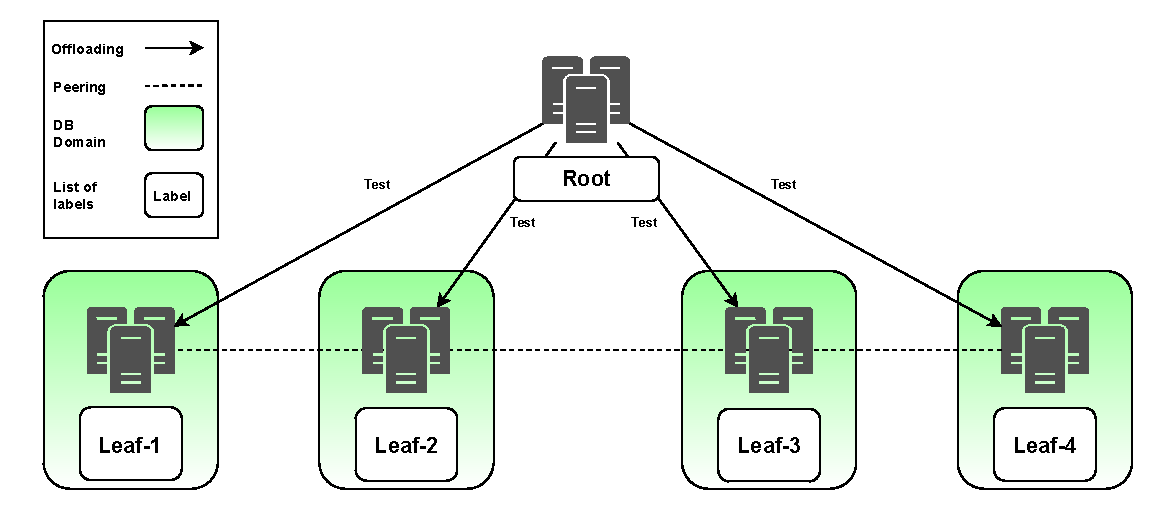
\includegraphics[scale=0.6]{Pictures/test}
\caption{Configuration test environment}\label{fig:test}
\end{figure}

\section{Latency}
In this section, the latency increase due to the overhead generated by Liqo technology will be evaluated using 4 virtual machines. One machine is consistently used as the secondary member (Root), while the others represent the primary member (Leaves). The maximum tolerated data communication latency for state estimation applications is approximately 1000 ms.

Typically, data, as depicted in Figure~\ref{fig:latency}, traverses about 4 clusters. The first two clusters usually consist of secondary stations, the third is the primary station overseeing the subnetwork of the two secondary stations, and the fourth is the Area Control Center containing the applications utilizing the data.

\begin{figure}[ht]\centering
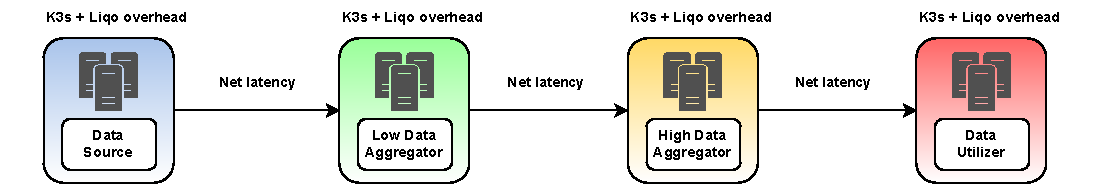
\includegraphics[scale=0.9]{Pictures/latency-schema}
\caption{Data flow from source to destination}\label{fig:latency}
\end{figure}

Therefore, the overall latency derives from the sum of Kubernetes + Liqo overhead for each individual cluster, plus the latencies of the networks connecting these clusters. The networks connecting these clusters typically consist of optical fiber networks for links between primary stations and Area Control Centers, and either fiber optic or radio links for the subnetwork of secondary stations.

According to the 2023 Development Plan of e-distribution~\cite{e2-1}, these networks include fiber optic cables illuminated with DWDM technology for connecting primaries to the control center, GPON fiber architectures, or 5G/LTE/4G radio links for connections between secondary and primary stations.

Let's consider the New AT/MT transformation station "Livigno" (SO) as presented in the 2023 development plan of e-distribuzione~\cite{e2-2}, as it represents an extreme case regarding the extension of the managed territory, approximately 400 km$^2$ in a rural environment. To estimate the network latency, we consider a fairly central location of the station within the area, hence the maximum distance between it and the secondary substations can be hypothesized to be about 30 km in the worst case. Over this distance, we consider a worst-case scenario of a 4G LTE network based on radio links, with cell towers approximately 5 km apart.

The network latency is calculated by adding the propagation speed over 30 km and the signal processing time for each cell tower. Assuming a signal processing time of about 20 ms and a propagation speed of 0.1 ms, the total latency would be 20 * 6 + 0.1 = 120.1 ms. For the distance between the primary station and its respective Area Control Center, a time of 1 ms can be assumed, as this technology operates at around tens of microseconds over 140 km. Therefore, the network latency considering one of the worst-case scenarios (use of radio links in a vast territory) can be approximated to about 122 ms, leaving a theoretical limit of 878 ms for the overhead of the technologies.

\subsection{Latency test}
Given that data in the architecture is transmitted using TCP protocols, which utilize acknowledgments (ACKs), latency is measured as the round-trip time of a packet. The tests were conducted using the ping command, with approximately 1000 iterations per test, individually executed from the Leaf machines to the Root machine.

Firstly, to establish a baseline for the tests, the network latency was calculated by averaging the mean of three ping values obtained from the virtual machines towards the root machine, as shown in the Table~\ref{t:2}. In this and the following tables, the arithmetic average will be calculated because every measures ah the same importance, and the avg standard deviation will be calculated using the formula~\eqref{eq:stddev} because tha data are uncorrelated:

\begin{equation} \label{eq:stddev}
\sigma_{\text{mean}} = \sqrt{\frac{\sum_{i=1}^{n} \sigma_i^2}{n}}
\end{equation}

where:
\begin{itemize}
  \item \(\sigma_i\) is the standard deviation of the value \(i\).
  \item \(n\) is the total number of values.
\end{itemize}

\begin{table}[ht]              
\centering 
\begin{tabular}{|l|c|c|}
\hline
\textbf{Virtual machine} & \textbf{Latency} & \textbf{\sigma} \\ 
\hline
Leaf-1 & 0.689 ms & 0.447 ms \\
\hline
Leaf-2 & 0.760 ms & 0.731 ms \\
\hline
Leaf-3 & 0.715 ms & 0.468 ms \\
\hline
Avg & 0.721 ms & 0.564 ms \\
\hline
\end{tabular}
\caption[Network average latency ]{Network average latency} \label{t:2}  
\end{table}

After establishing the network latency, we proceed to calculate the latency between a pod located on different Leaf nodes and a pod in the Root node, where the Leaf nodes and the Root node belong to the same cluster, shown in Table~\ref{t:3}, or belong to different clusters peered with Liqo, shown in Table~\ref{t:4}.

\begin{minipage}{0.45\textwidth}
  \centering
  \vspace{0.5cm}
  \begin{tabular}{|l|c|c|}
  \hline
  \textbf{Cluster Node} & \textbf{Latency} & \textbf{\sigma}  \\ 
  \hline
  Leaf-1 & 0.735 ms & 0.294 ms \\
  \hline
  Leaf-2 & 0.992 ms & 0.568 ms \\
  \hline
  Leaf-3 & 0.936 ms & 0.483 ms \\
  \hline
  Avg & 0.888 ms & 0.463 ms \\
  \hline
  \end{tabular}
  \captionof{table}{Latency between pod on different nodes, but on the same cluster}
  \label{t:3}\vspace{0.5cm}
\end{minipage}%
\hspace{0.05\textwidth} % Adjust the horizontal space between the tables
\begin{minipage}{0.45\textwidth}
  \centering
  \vspace{0.5cm}
  \begin{tabular}{|l|c|c|}
  \hline
  \textbf{Remote Node} & \textbf{Latency} &  \textbf{\sigma} \\ 
  \hline
  Leaf-1 & 1.269 ms & 0.724 ms \\
  \hline
  Leaf-2 & 1.400 ms & 0.829 ms \\
  \hline
  Leaf-3 & 1.368 ms & 0.903 ms \\
  \hline
  Avg & 1.346 ms & 0.822 ms\\
  \hline
  \end{tabular}
  \captionof{table}{Latency between pod on different clusters, peered with Liqo}
  \label{t:4}\vspace{0.5cm}
\end{minipage}

The increase due to Liqo is measured by subtracting the average latency from Table~\ref{t:3}, which is the sum of network latency + Kubernetes overhead, from the average latency shown in Table~\ref{t:4}, which is the sum of network latency + Kubernetes overhead + Liqo overhead. This calculation yields the result shown in Table~\ref{t:5}. 

The result shows that the overhead added by Liqo is negligible compared to the total tolerated latency of 1000 ms, as well as compared to one of the worst-case scenarios such as the Livigno case.

\begin{table}[ht]              
\centering 
\begin{tabular}{|l|c|}
\hline
\textbf{Average Liqo Latency} & \textbf{\sigma}\\ 
\hline
0.458 ms  & 0.679 ms \\
\hline
\end{tabular}
\caption{Average Liqo Latency} \label{t:5}  
\end{table}

The latency between pods on different Kubernetes clusters without multi-cluster technologies was not tested, as the goal is to demonstrate the latency increase using Liqo across different clusters compared to using a single Kubernetes cluster connecting all nodes.

\section{k3s reaction time}

In the upcoming test, two clusters of virtual machines connected via unidirectional Liqo peering were utilized: the consumer cluster and the provider cluster. The objective was to show the consumer cluster's response time in the event of disconnection of the virtual node representing the provider cluster, for any reason.

The test involved two scripts. The first script disabled the network interface on the virtual machine running Liqo in the provider cluster and recorded the timestamp. The second script executed a loop on the consumer cluster, running 'kubectl get node' every 0.4 seconds, and appending the output with a timestamp. (A shorter interval wasn't feasible due to the command execution time.)

The results are depicted in Graph~\ref{graph:k-reaction}. Comparing these results with findings from previous thesis~\cite{e3-1} about the local solution using only Kubernetes, which utilized virtual machines running on different physical machines with slightly different parameter settings, it is evident that the order of magnitude remains consistent. This indicates that the introduction of Liqo technology does not add noteworthy delays compared to the typical delays of a straightforward Kubernetes architecture.

\begin{figure}[ht]\centering
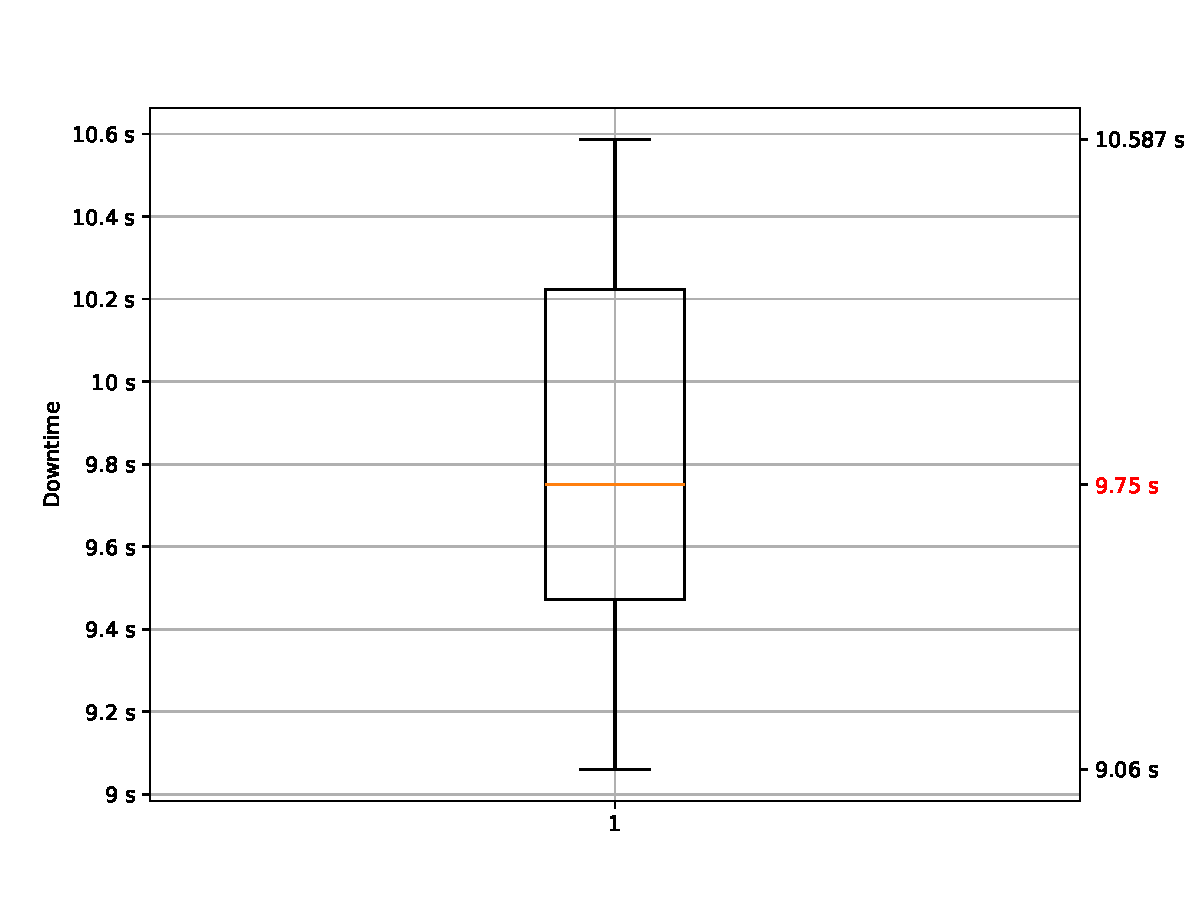
\includegraphics[scale=0.5]{Pictures/k3s-reaction}
\caption{Reaction to set virtual node as Not Ready in case of remote cluster disconnession.}\label{graph:k-reaction}
\end{figure}

Moreover, using the same machines but connecting them through a single Kubernetes server and utilizing identical parameter settings, it was observed that the cluster response time in the event of a node failure is slightly higher by a few seconds compared to the time required to detect a node failure representing a Liqo cluster, as depicted in Figure~\ref{graph:k-reaction2}. This difference stems from the Virtual Kubelet's unique management and health check optimization implemented by Liqo, which supersedes traditional kubelet functions for the virtual node management.

\begin{figure}[ht]\centering
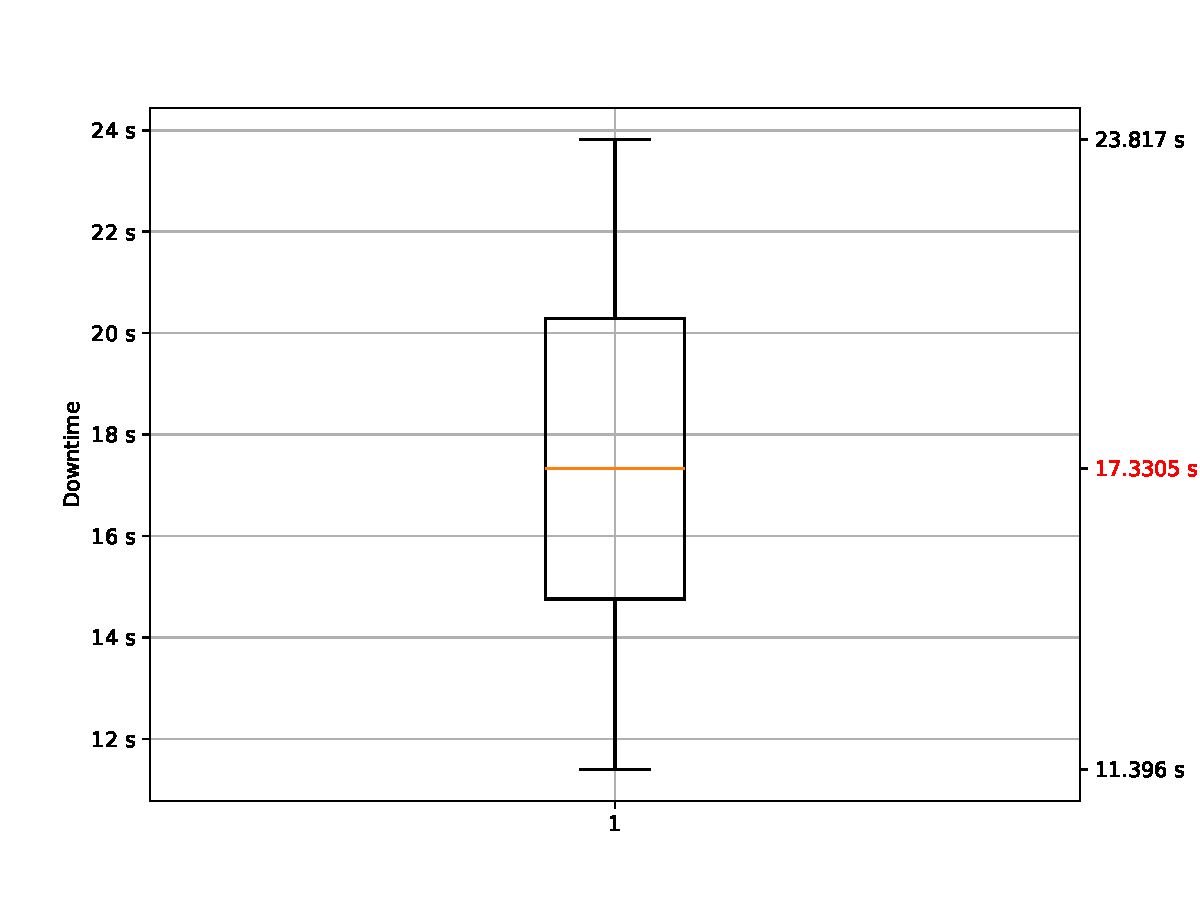
\includegraphics[scale=0.5]{Pictures/k3s-reaction2}
\caption{Reaction to set virtual node as Not Ready in case of local node disconnession.}\label{graph:k-reaction2}
\end{figure}

\section{Stream reaction time}
The following tests demonstrate the downtime of a data stream from a PMU in the following scenarios:

\begin{enumerate}
\item Internal failure of a PDC pod, resulting in the rescheduling of the application. 
\item Fault/disconnection of the cluster hosting a PDC pod, resulting in the application being rescheduled to another cluster.
\end{enumerate}

Downtime is calculated from the timestamp of the last data frame of the old stream to the timestamp of the first data frame of the new stream, encompassing the time required for rescheduling the PDC pod, retrieving configurations from the database system, and reconnecting to the data stream.

These tests examine a data stream originating from a PMU that traverses through two PDC pod, one considered low-level and the other considered high-level, before reaching its intended application. The use of the data frame timestamp is crucial due to the PMU's real-time production of data frames at 33-millisecond intervals, ensuring precise downtime calculations and analysis.

\subsection{Pod failure}
The failure scenario of the PDC pod was simulated by customizing the liveness probe mechanism, intentionally triggering a failure check after the pod had been running for 60 seconds. The pod was located in a remote cluster managed by Liqo.

The test results, displayed in Graph~\ref{graph:pod-down}, illustrate the median duration required for the lower-level PDC application to resume normal operation. This duration encompasses the time from detecting the PDC pod failure to its subsequent recovery, including the processes of restarting the pod, retrieving configurations from the system database, and re-establishing connection to the data stream.

Comparing these results with findings from previous thesis~\cite{e3-1} about the local solution using only Kubernetes,  where the pod recovery time ranged between 17-25 seconds, it is noted that here too, despite slight differences of a few seconds primarily due to environmental variables such as machine power, the order of magnitude remains consistent. 

\begin{figure}[ht]\centering
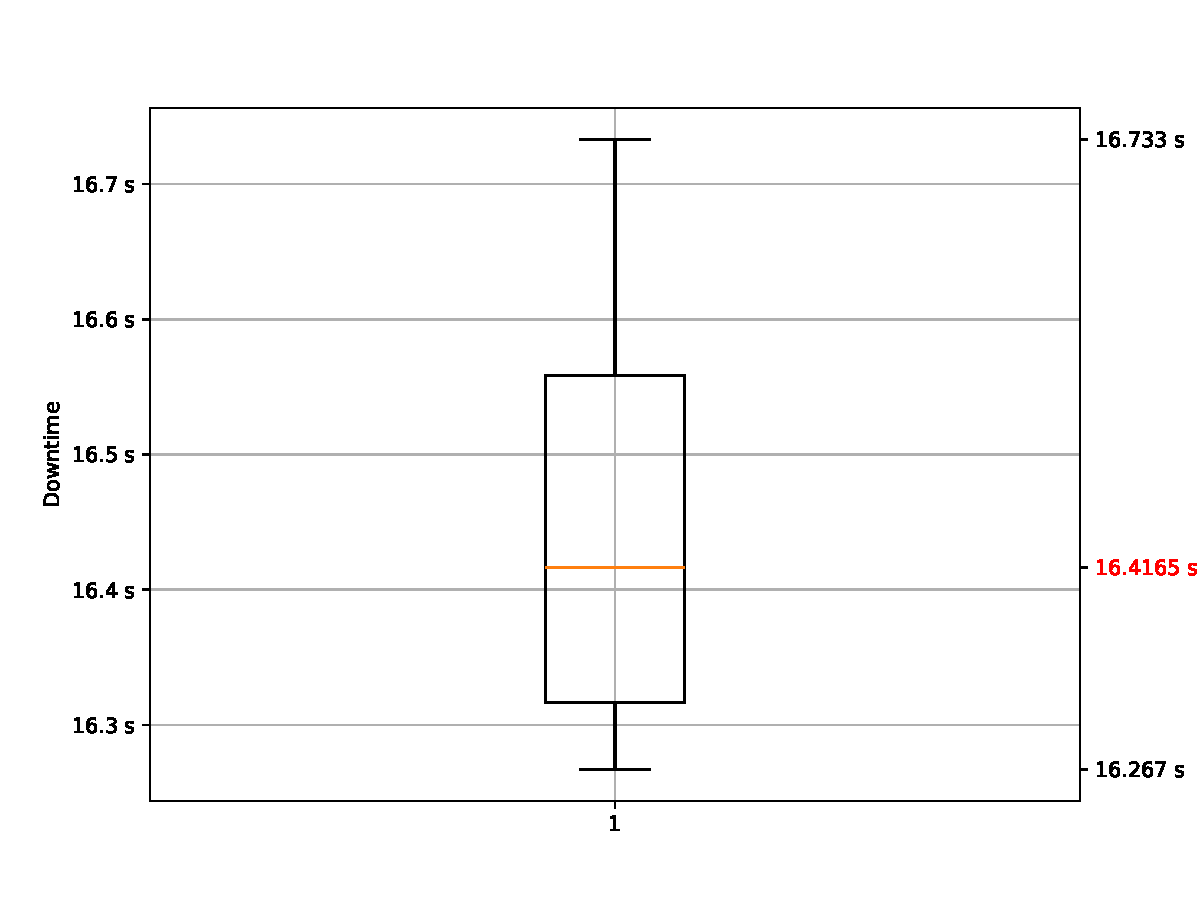
\includegraphics[scale=0.5]{Pictures/pdc-pod-down}
\caption{Box plot regarding stream downtime from last old data to the first new data in case of pod failure.}\label{graph:pod-down}
\end{figure}

\subsection{Cluster failure}
The failure scenario was simulated by deliberately disabling the network interface of the lower-level PDC pod within the cluster. The deployment configuration of the lower-level PDC includes specific affinities to ensure that in the event of rescheduling, it can only be placed on another leaf cluster. As depicted in Figure~\ref{fig:test}, these leaf clusters are also managed by Liqo.

\begin{figure}[ht]\centering
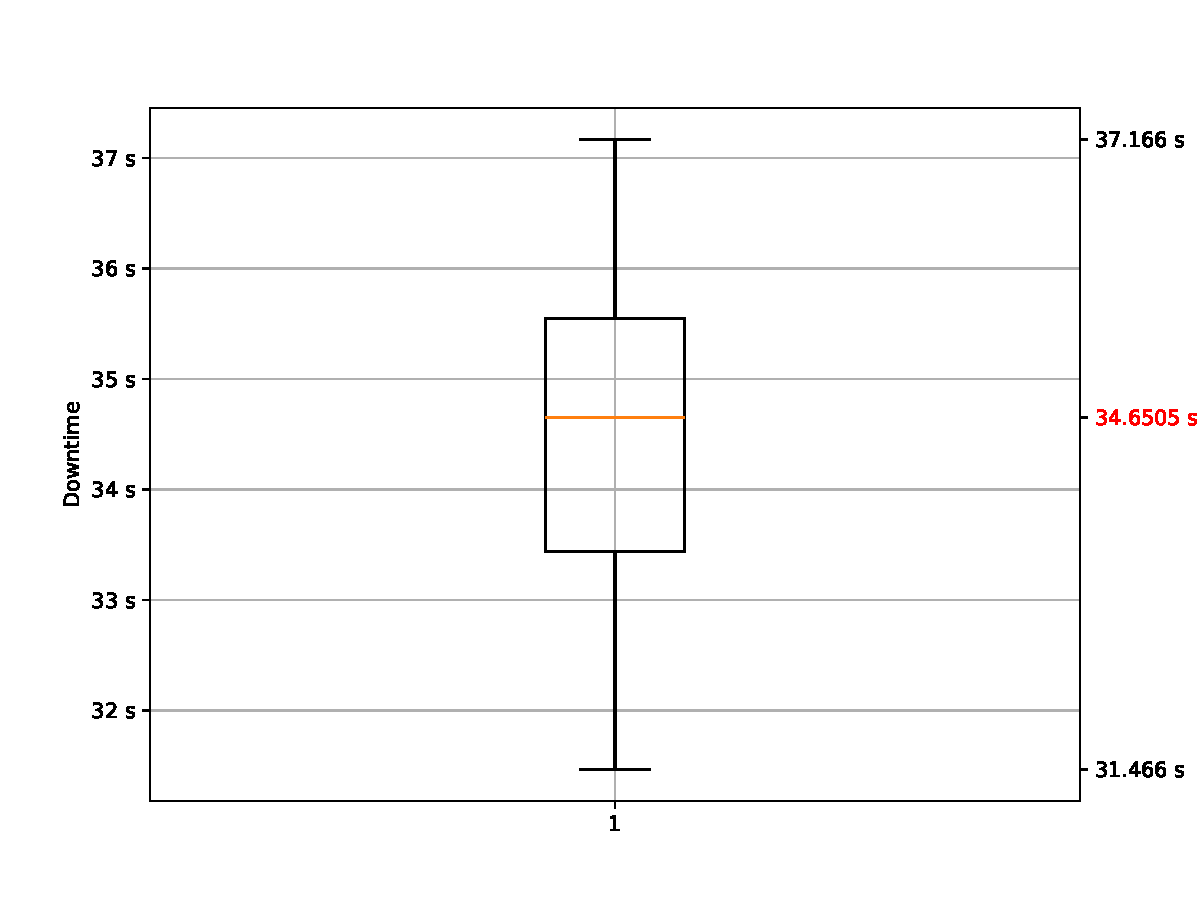
\includegraphics[scale=0.5]{Pictures/pdc-cluster-down}
\caption{Box plot regarding stream downtime from last old data to the first new data in case of cluster failure.}\label{graph:cluster-down}
\end{figure}

The test results, displayed in Graph~\ref{graph:cluster-down}, illustrate the median duration required for the lower-level PDC application to resume normal operation. This duration includes the time required for the cluster to detect that the virtual node hosting the PDC is unreachable (9.75 seconds as shown in Graph~\ref{graph:k-reaction}), the waiting time before it can be rescheduled to another node (5 seconds as indicated in table \ref{t:1}), and the time necessary for the pod to restart (16.41 seconds as depicted in Graph~\ref{graph:pod-down}).

Comparing the results with the values shown in Figure ~\ref{fig:seba}, illustrating findings from the previous thesis~\cite{e3-1} focusing on the local solution using only Kubernetes, it is observed that the order of magnitude remains consistent. This reaffirms alongside previous tests that the introduction of Liqo technology does not introduce significant changes in terms of architectural overhead. In fact, in some cases, such as the optimization of the Kubelet, it enables better performance compared to the traditional Kubernetes architecture.


\begin{figure}[ht]\centering
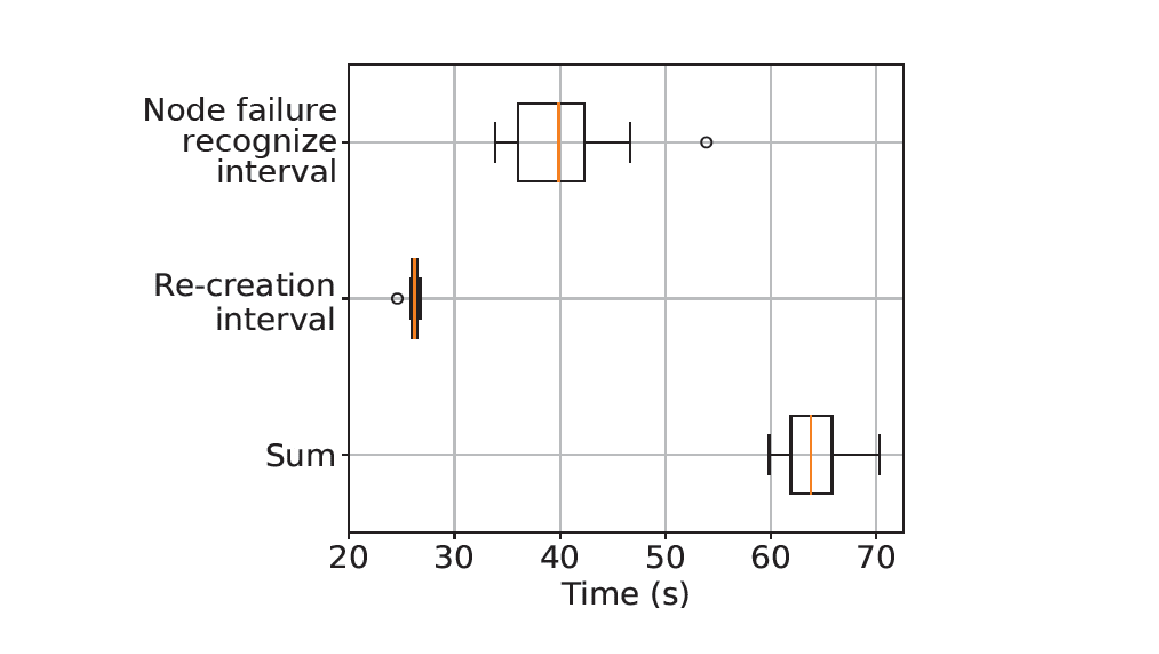
\includegraphics[scale=0.5]{Pictures/seba}
\caption{Time required to recover services on a disconnected node, on a traditional kubernetes cluster.}\label{fig:seba}
\end{figure}

\section{Overall evaluation}
In this section, we summarize the findings from the various tests conducted to evaluate the performance, reliability, and resilience of the logical domain grouping implementation using Crownlabs and Liqo technology. The following points encapsulate the overall evaluation:

\begin{itemize}
\item \textbf{Test Environment and Configuration:} The test environment, meticulously configured using Crownlabs and Kubernetes clusters, accurately simulated real-world scenarios. The use of low-capacity virtual machines reflects typical setups in energy monitoring and distribution stations, ensuring relevance and applicability of the results. 

The fully-meshed star topology with a central root cluster efficiently managed the workload distribution and ensured robustness in case of node or cluster failures. The unidirectional peering for distributed database operations, as implemented through Liqo, facilitated seamless resource sharing and enhanced system reliability.

\item \textbf{Latency Analysis:} The latency tests revealed that the additional overhead introduced by Liqo technology is minimal. The measured average Liqo latency of 0.458 ms is well within acceptable limits for state estimation applications, which tolerate up to 1000 ms. This demonstrates that Liqo can be effectively utilized in distributed systems without significantly impacting communication performance.

\item \textbf{K3s Node Reaction Time:} The reaction time tests indicated that the introduction of Liqo technology did not introduce substantial delays. In fact, the Liqo-managed virtual kubelet demonstrated optimized health checks and node management, resulting in slightly faster response times in certain failure scenarios compared to traditional Kubernetes setups.

\item \textbf{Stream Reaction Time:} The tests simulating pod and cluster failures demonstrated that the downtime for resuming data streams was comparable to, if not slightly better than (in the case of cluster failure), traditional Kubernetes-only environments. This, along with new features such as the temporary independent management of a part of the network (with the continuation of the data stream inside) and the optimization of control capacity by a central entity to manage the rescheduling of the aggregator on other clusters, illustrates the significant advantages of introducing Liqo technology.

\item \textbf{Reliability and Resilience:} Overall, the tests conducted on the logical domain grouping architecture have demonstrated its high resilience against both internal and external cluster failures. Throughout the testing process, there was not a single instance where the system failed to automatically converge to a new stable state after a fault was introduced. Moreover, in scenarios where a cluster became disconnected, the system reliably reintegrated the cluster into the architecture automatically once the connection was restored. This seamless reintegration highlights the robustness and efficiency of the architecture in maintaining operational continuity and stability, underscoring the significant advantages of adopting this approach.

\item \textbf{Scalability and Flexibility:} The modular setup of clusters and the dynamic nature of Liqo peering allow for a high degree of adaptability, enabling the inclusion or exclusion of clusters without compromising the entire architecture. This is crucial for evolving system requirements and expanding infrastructure without significant overhauls. Scalability remains anchored to the official limits present in the Kubernetes documentation, although it has increased considerably since the set of nodes within a cluster is perceived as a single virtual node.

\item \textbf{Comparison with Traditional Kubernetes:} Throughout the evaluations, it was evident that the logical domain grouping implementation leveraging Liqo provided performance metrics on par with those of traditional Kubernetes architectures. Additionally, the introduction of Liqo offers several benefits, such as isolated operation in case of disconnections, enhanced central control over the entire network, and the ability to manage cluster failures that a Kubernetes-only architecture cannot easily implement.
\end{itemize}

In conclusion, the analyses confirm that the chosen implementation of logical domain grouping  offers a robust, scalable, and efficient solution for managing distributed systems. The minimal overhead introduced by Liqo, coupled with its advanced features, makes it a valuable addition to Kubernetes-based infrastructures, ensuring high resilience and optimal performance.
